\subsection{Sim City 2000}
Sim City 2000 ist ein im Jahr 1993 erschienenes Städteaufbauspiel für Einzelspieler, welches in das Genre \textit{Simulation} fällt \cite{simcity:ea}. Das Spiel wurde ursprünglich von \textit{Maxis} für den Mac entwickelt und publiziert, wurde in den kommenden Jahren jedoch für weitere Konsolen herausgegeben, darunter \textit{SNES, PlayStation} und \textit{Nintendo 64}. Im Jahr 2005 erschien es schließlich für den PC unter Windows \cite{simcity:igdb}. Der Spieler startet auf einer ausgewählten Karte, welche ein \textit{Square Grid} mit verschiedenen Höhen und Terrain besitzt. Die dabei zentrale Ressource ist Geld in Form von US Dollars. Der Spieler kann mit diesem Geld aus einer breiten Palette an Gebäuden wählen, darunter \textit{Schulen, Bibliotheken, Krankenhäuser} und \textit{Kraftwerke} \cite*[]{simcity:igdb}, welche die Bedürfnisse der Einwohner befriedigen und für Recht und Ordnung in der Stadt sorgen. Diese Gebäude besitzen einen Radius, was ein weiteres strategisches Element dieses Spiels darstellt, da auf möglichst sinnvolles Platzieren der jeweiligen Gebäude geachtet werden muss. Für Wohn-, Industrie- und Kaufhausgebäude markiert der Spieler Zonen, statt die Gebäude einzeln zu setzen. Die Gebäude dieser Zonen werden dann, je nach Bedarf, Stück für Stück aufgebaut oder wieder verlassen. Der Bedarf jeweiliger Zonen ist in \autoref{image:simcity} anhand des grünen (Wohngebäude), des blauen (Kaufhausgebäude) und des gelben (Industriegebäude) Balkens am linken Auswahlbalken erkennbar. Zeigt ein Balken dabei in die Richtung des \textit{+}, so signalisiert das \textit{Bedarf}, zeigt der Balken jedoch in die Richtung des \textit{-}, ist \textit{Überschuss} vorhanden. Zwischen diesen Zonen herrscht eine Relation, so benötigen Kaufhausgebäude die Industriegebäude als Produktionsquelle, und Wohngebäude als Käufer. Die Wohngebäude wiederum benötigen Arbeitsplätze, sowohl in Kaufhausgebäuden als auch in Industriegebäuden. Die Industriegebäude benötigen die Arbeitskräfte der Wohngebäude und Abnehmer für die produzierte Ware in Form von Kaufhausgebäuden. Diese Relation wird wie folgt berechnet (R:C:I beschreibt die Relation zwischen Wohngebäuden zu Kaufhausgebäuden zu Industriegebäuden): 
\newpage
\begin{itemize}
    \item Unter 10.000 Einwohnern: R:C:I = 4:1:3
    \item Zwischen 10.000 und 60.000 Einwohnern: R:C:I = 4:2:2
    \item Über 60.000 Einwohner: R:C:I = 4:3:1 \cite*[]{simcity:somacon}
\end{itemize}
Die Wohngebäude brauchen \textit{Strom, Wasser, Bildung, Sicherheit} und \textit{Freizeitaktivitäten}, welche allesamt durch platzierbare Gebäude gegeben werden können. Bildung ist eine Kernkomponente des Spiels, denn je nach Bildungsgrad der Stadt steigt oder fällt die Kriminalitätsrate und entscheidet auch darüber, welche Industrien blühen oder bankrottgehen. Der Bildungsgrad wird gemessen am EQ (\textit{education quotient}), so erhöht beispielsweise eine Schule den EQ von den 5 bis 20 Jahre alten Bewohnern. Es gibt insgesamt 156 Gebäude, welche in 8 Kategorien eingeteilt werden können, darunter verschiedene Arten von Wohngebäuden, Kaufhausgebäuden oder Industriegebäuden, wie auch verschiedene Parks, Statuen oder Kraftwerke \cite*[]{simcity:fandom}. \\
Ein weiteres zentrales Element des Spiels ist das \textit{Budget}, welche am Ende jedes Spieljahres adjustiert werden kann. So kann man die \textit{Steuern} erhöhen, die die Einwohner zahlen müssen, wie auch die \textit{Ausgaben} für verschiedene Institutionen anpassen. So kann beispielsweise das Budget der Polizei verringert werden oder das Budget der Feuerwehr erhöht werden, woraus jeweils Effektivitätsboni oder -mali folgen \cite*[]{simcity:video}. \\
Das Spiel hat keine Siegbedingungen, die Ziele setzt sich der Spieler selber. Mögliche Ziele sind dabei eine möglichst schöne Stadt, eine Stadt mit möglichst vielen Einwohnern oder man spielt vor sich hin und versucht ein Problem nach dem anderen zu lösen. Auch wenn das Spiel an sich nicht gewonnen werden kann, gibt es dennoch einen Endzustand und eine Art Gewinnsequenz. Der Endzustand ist ein Game Over, bei dem der Spieler durch \$100.000 Dollar Schulden aus \glqq seinem Büro eskortiert wird\grqq, siehe \autoref{image:simcitygameover}. Die mögliche Gewinnsequenz, die einem Sieg am ehesten kommt, ist durch baubare Arkologien bedingt. Arkologien sind sich selbst erhaltende Städte mit einer hohen Bevölkerungsdichte innerhalb eines meist hohen Gebäudes. Der Begriff wurde in den 50er Jahren von dem italienisch-amerikanischen Architekten Paolo Soleri geprägt, jedoch wurde bis heute noch keine echte Arkologie gebaut, auch wenn es dazu bereits einige Experimente, beispielsweise in Arizona, gibt \cite*[]{misc:arcology}. Nachdem der Spieler 301 sogenannte \textit{launch arcos} gebaut hat und das Jahr 2051 bereits angebrochen wurde, erscheint dem Spieler eine Nachricht, in Englisch \textit{\glqq The Exodus has begun\grqq}, woraufhin alle gebauten Arkologien explodieren und dem Spieler suggeriert wird, die Schiffe wären aufgebrochen, um neue Planeten zu besiedeln \cite*[]{simcity:arcology}. \\
Auch wenn das Spiel ein reines \textit{Singleplayer} Game ist, also lediglich ein menschlicher Spieler gleichzeitig spielen kann, spielt man dennoch gegen max. vier weitere Computerspieler, auch genannt \textit{KIs} (Künstliche Intelligenzen). Die maximal vier weiteren angrenzenden Karten der jeweils zu Anfang ausgewählten Karte werden von \textit{KIs} besiedelt und ebenfalls bebaut. Diese Nachbarstädte können mittels gegebener Transportmöglichkeiten, zum Beispiel Flugzeug oder Zug, Gewinn bringen, da die Bewohner der Nachbarstädte in beispielsweise den Kaufhäusern Geld ausgeben \cite*[]{simcity:manual}. \\
Eine weitere Eigenheit des Spiels sind die sogenannten \textit{Katastrophen} beziehungsweise \textit{Desaster}. Diese können vom Spieler komplett ausgeschaltet werden, falls gewollt. Die meisten Desaster können zufällig und natürlich passieren, darunter Feuer, Aufstände oder Fluten. Alle Desaster können ebenfalls vom Spieler selbst initiiert werden, um die Grenzen der eigenen Stadt auf die Probe zu stellen. Manche Katastrophen sind verkettet, so können Aufstände zu Feuer führen, oder Erdbeben zur Explosion von Kernkraftwerken führen, welche wiederum zu Feuern und Aufständen führen kann \cite*[]{simcity:manual}.\\
Das Spiel hatte einen Vorgänger \textit{Sim City}, welcher bereits 1989 erschien, und erhielt neun Nachfolger, darunter \textit{Sim City 3000, Sim City 4} und den neusten Teil \textit{SimCity: BuildIt}, welcher lediglich für mobile Endgeräte verfügbar ist und 2014 erschien. Der letzte Teil für den Computer erschien 2013 und trägt den Titel \textit{SimCity 2013} \cite*[]{simcity:timeline}. \\ Wichtige Eckdaten sind in \autoref{table:simcity} vorzufinden.

\paragraph*{Ressourcen}
\begin{itemize}
    \item Dollar
\end{itemize}
\newparagraph{Rezensionen}
\begin{tabularx}{0.8\textwidth} { 
    | >{\raggedright\arraybackslash}X 
    | >{\centering\arraybackslash}X 
    | >{\raggedleft\arraybackslash}X | }
    \hline
    IGDB & 78\% \cite*[]{simcity:igdb}\\
    \hline
    AllGame & 4.5/5 (PC) \cite*[]{simcity:review:allgame}\\
    \hline
    MacUser & 4.5/5 (Mac) \cite*[]{simcity:review:macuser}\\
    \hline
    Sega Saturn Magazine & 86\% (SAT) \cite*[]{simcity:review:segasaturn}\\
    \hline
\end{tabularx}

\begin{table}[]
    \centering
    \caption{Sim City 2000 Eigenschaften (\cite*[]{simcity:igdb})}
    \label{table:simcity}
    \begin{tabular}{|l|l|}
    \hline
    Erscheinungsjahr & 1993                                                                           \\ \hline
    Entwickler       & Maxis                                                                      \\ \hline
    Publisher        & Maxis                                                                      \\ \hline
    Multiplayer      & Nein                                                                           \\ \hline
    Ressourcen       & Dollars \\ \hline
    Siegbedingungen  & Keine                                               \\ \hline
    Endzustände  & Game Over                                               \\ \hline
    Perspektive      & Isometrisch                                                                          \\ \hline
    \end{tabular}
\end{table}

\begin{figure}
    \begin{center}
        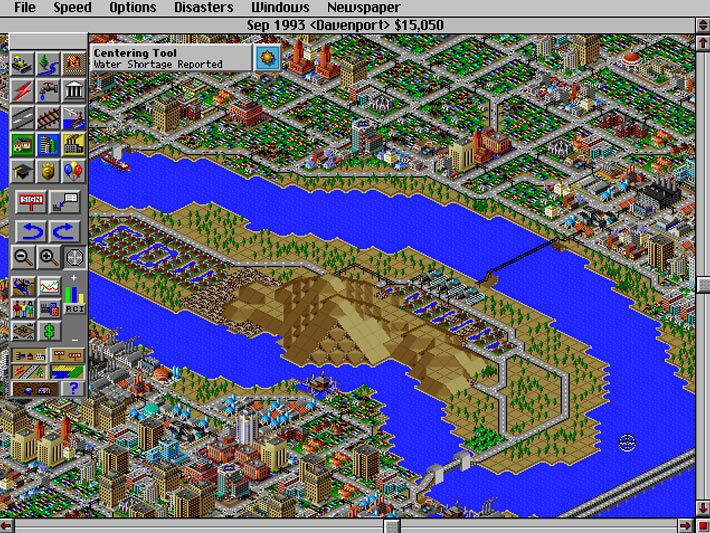
\includegraphics[width=300px]{0.bilder/simcity.jpg}
    \end{center}
    \caption{Screenshot aus Sim City 2000 (\cite{simcity:igdb})} \label{image:simcity}
\end{figure}
\begin{figure}
    \begin{center}
        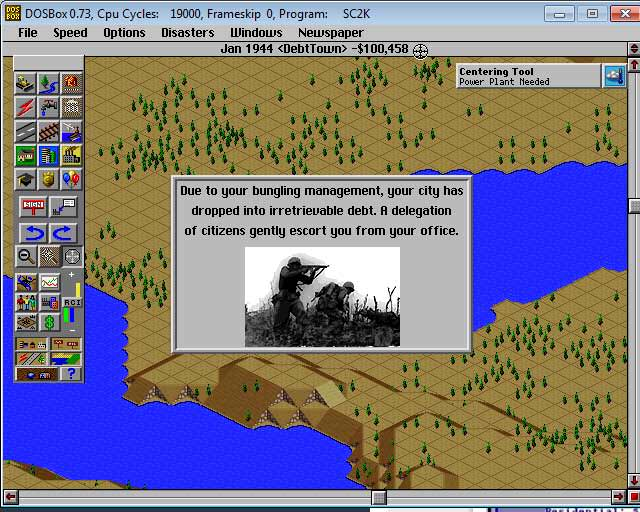
\includegraphics[width=300px]{0.bilder/simcityend.jpeg}
    \end{center}
    \caption{Game Over in Sim City 2000 (\cite{simcity:gameover})} \label{image:simcitygameover}
\end{figure}